%% Generated by make_supplement.py from supplement_body.tex and numbers/*.json; edit those, not this file.
%% Supplementary material for the ESN paper. Tables are inserted by make_supplement.py from numbers/*.json.
\documentclass[aip,cha,preprint,amsmath,amssymb,longbibliography]{revtex4-2}
\usepackage{graphicx}
\usepackage{bm}
\usepackage{xcolor}
\usepackage[colorlinks=true,linkcolor=blue!55!black,citecolor=blue!55!black,urlcolor=blue!55!black]{hyperref}
\newcommand{\Uin}{U_{\mathrm{in}}}
\renewcommand{\thefigure}{S\arabic{figure}}
\renewcommand{\thetable}{S\arabic{table}}
\renewcommand{\thesection}{S\arabic{section}}

\begin{document}

\title{Supplementary material for ``Do trained models keep attractors hidden? Forced spurious equilibria and a survival law
for hiddenness''}
\author{Maksim Elisov}
\affiliation{Samara National Research University, Moskovskoye Shosse 34, Samara 443086, Russia}
\maketitle

All statistics pool the six regimes whose hidden attractors are hidden in the strict sense; LE1 is shown separately where
noted. Notation, ensembles and protocols are those of the main text. The numbers come from the analysis scripts
\texttt{paper\_hetero.py}, \texttt{paper\_fidelity.py} and \texttt{paper\_completeness.py} of the data archive.

\section{Survival by regime}

Figure~\ref{fig:sm_regime} shows the survival curves of every regime, and Table~\ref{tab:sm_slopes} the slope of the
logistic fit per regime. The slopes differ significantly between regimes in all ensembles: likelihood ratio for the
regime~$\times\log(1+U)$ interaction $23.3$ ($p=3\times10^{-4}$) in the size sweep, $14.1$ ($p=0.015$) and $22.0$
($p=5\times10^{-4}$) for the full-protocol ensemble counted by $U$ and by $\Uin$, and $36.8$ ($p=7\times10^{-7}$) for the
other classes. The differences are about a factor of two (classes: from $-2.7$ in SE11 to $-5.4$ in Wang--Chen at
$a=0.006$), whereas the heuristic $\Pr(\text{hidden}\mid U)\approx(1-p_B)^{\nu U}$ of the main text predicts slopes
proportional to $\log(1-p_B)$, which spans a factor of $210$ across regimes in the size sweep ($0.0055$ to $1.16$) and $24$ for
the classes. The implied $\nu$ ranges from $0.12$ to $57$ (size sweep) and from $0.59$ to $6.2$ (classes), and a common $\nu$
is rejected (likelihood ratio $44.8$ and $497$). In Chua~I, where the network basin covers $0.12$ of the reservoir cube, the
slope of the log-linear model is $-0.015\pm0.025$ per unstable equilibrium. The curve is therefore a regularity in $U$ with
regime-dependent steepness, not a consequence of the basin size alone.

\begin{table*}
\caption{Slope of $\log(1+U)$ (or $\log(1+\Uin)$) per regime, logistic regression with the covariates of the main fits
(maximum likelihood, model standard errors). In the Wang--Chen regime at $a=0.006$ no echo state network with $U\ge1$
keeps the attractor hidden, so the slope diverges (complete separation); the Firth estimate is given instead. The last rows
give the common slope and the likelihood-ratio test of regime-specific slopes.}
\label{tab:sm_slopes}
\begin{ruledtabular}
\begin{tabular}{llll}
Regime & ESN, size sweep, $U$ & ESN, full protocol, $\Uin$ & mlp, mlp2, res, $\Uin$ \\
\hline
SE3 & $-4.51\pm1.01$ & $-2.51\pm0.45$ & $-4.08\pm0.50$ \\
SE11 & $-3.41\pm0.83$ & $-4.70\pm0.88$ & $-2.66\pm0.30$ \\
WC & $-\infty$ (Firth $-6.8$) & $-\infty$ (Firth $-6.4$) & $-5.42\pm0.43$ \\
WC$'$ & $-4.24\pm1.26$ & $-5.59\pm1.19$ & $-3.57\pm0.28$ \\
Chua~I & $-0.71\pm0.50$ & $-5.00\pm1.84$ & $-3.57\pm0.31$ \\
Chua~II & $-2.45\pm1.75$ & $-1.44\pm0.75$ & $-4.59\pm0.35$ \\
\hline
common slope & $-3.08\pm0.40$ & $-3.54\pm0.35$ & $-3.94\pm0.15$ \\
interaction LR $\chi^2$ (5 df) & $23.3$, $p=0.0003$ & $22.0$, $p=0.0005$ & $36.8$, $p=7e-07$ \\
\end{tabular}
\end{ruledtabular}
\end{table*}


\begin{figure*}
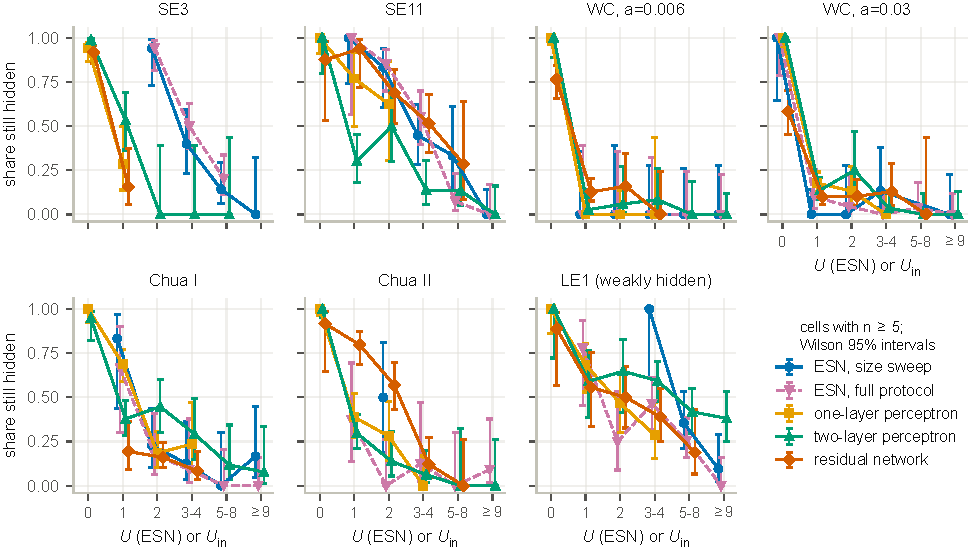
\includegraphics[width=\textwidth]{figures/sm_regime_survival.pdf}
\caption{Survival against the number of unstable equilibria per regime: echo state networks of the size sweep and of the
full-protocol ensemble (counted by $U$) and one-layer perceptrons, two-layer perceptrons and residual networks (counted by
$\Uin$). Cells with at least five pairs, Wilson $95\%$ intervals. LE1, whose attractor is only weakly hidden, is shown for
comparison.}
\label{fig:sm_regime}
\end{figure*}

\section{Regime mix, clustering and standardization}

Pooled curves mix regimes whose composition differs between bins. In the size sweep $30$ of the $49$ pairs with $U=1$ come
from the two Wang--Chen regimes, where no attractor survives, which produces the dip of the pooled curve at $U=1$.
Figure~\ref{fig:sm_std} compares the crude curves with two standardized ones. Direct standardization reweights the
regime cells of each bin to the overall regime mix; it is unstable where cells are small. Model-based standardization
averages the fitted regime-specific survival over a fixed regime mix and removes the dip: $0.60$ $[0.49,0.68]$ at $U=1$ and
$0.45$ $[0.38,0.52]$ at $U=2$ in the size sweep, $0.58$ $[0.49,0.65]$ and $0.44$ $[0.40,0.50]$ in the full-protocol
ensemble. For the other classes crude and standardized curves nearly coincide.

Almost every model contributes one pair (size sweep: $381$ pairs from $380$ networks; classes: $3329$ pairs from $3284$
models), so Wilson intervals on pairs are close to cluster-bootstrap intervals over models (Fig.~\ref{fig:sm_std}). The
slopes of the main fits with model, cluster-robust and cluster-bootstrap ($2000$ replicates) errors are
$-3.08\pm0.40$, $\pm0.69$ and $\pm0.74$ (interval $[-4.89,-2.04]$) for the size sweep, $-4.25\pm0.42$, $\pm0.60$ and $\pm0.65$
($[-5.74,-3.27]$) for the full-protocol ensemble counted by $U$, $-3.54\pm0.35$, $\pm0.45$ and $\pm0.49$ counted by $\Uin$,
and $-3.94\pm0.15$, $\pm0.16$ and $\pm0.16$ ($[-4.27,-3.67]$) for the classes. With a single pair per cluster the
cluster-robust error is a heteroskedasticity-robust error, and its excess over the model error reflects the misfit of a
common slope.

\begin{figure*}
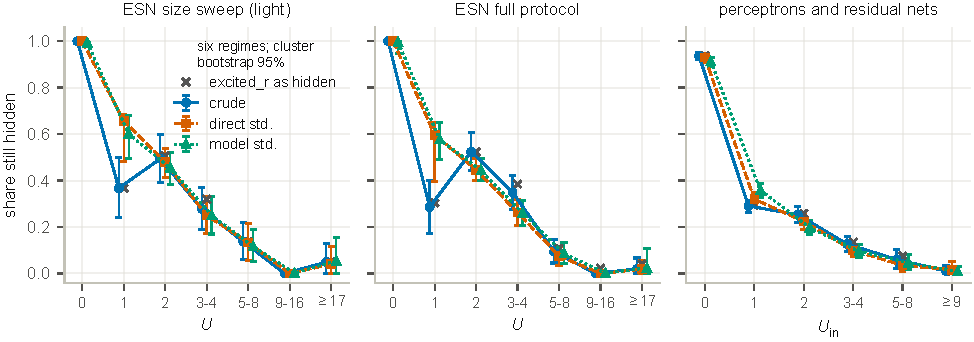
\includegraphics[width=\textwidth]{figures/sm_standardized.pdf}
\caption{Pooled survival curves, crude (cluster-bootstrap $95\%$ intervals), directly standardized and model-based
standardized to the overall regime mix; crosses: crude curve with attractors excited only at a finite radius counted as
hidden.}
\label{fig:sm_std}
\end{figure*}

\section{Form of the dependence}

Table~\ref{tab:sm_links} and Fig.~\ref{fig:sm_links} compare the logit in $\log(1+U)$ with a logit in $U$, a log link in $U$
(the form suggested by the heuristic), and complementary log-log links in $U$ and in $\log(1+U)$. The logit in $\log(1+U)$ has
the lowest AIC in all eight comparisons, on all pairs and on pairs with at least one unstable equilibrium; the log link in $U$
comes next, with slopes of $-0.20$, $-0.31$ and $-0.68$ per unstable equilibrium in the size sweep, the full-protocol
ensemble and the classes. A complementary log-log link in $\log U$ on pairs with $U\ge1$ estimates the exponent $c$ in
$\Pr(\text{hidden})=\exp(-aU^c)$, with $c=1$ for independent equilibria: $c=0.59\pm0.25$ (size sweep), $0.97\pm0.37$ and
$0.87\pm0.28$ (full protocol, $U$ and $\Uin$), none different from one, and $0.77\pm0.08$ for the classes, below one.

\begin{table}
\caption{Difference of AIC to the best model for five links and transformations of the count, on all reproduced pairs and on
those with at least one unstable equilibrium (second column of each ensemble). Covariates as in the main fits.}
\label{tab:sm_links}
\begin{ruledtabular}
\begin{tabular}{lcccccc}
 & \multicolumn{2}{c}{ESN sweep} & \multicolumn{2}{c}{ESN full} & \multicolumn{2}{c}{classes} \\
Model & all & $\ge1$ & all & $\ge1$ & all & $\ge1$ \\
\hline
logit, $\log(1+U)$ & 0.0 & 0.0 & 0.0 & 0.0 & 0.0 & 0.0 \\
logit, $U$ & 65.4 & 31.3 & 60.4 & 22.6 & 221.7 & 17.4 \\
log link, $U$ & 50.2 & 11.9 & 72.5 & 9.6 & 322.9 & 46.1 \\
cloglog, $U$ & 96.1 & 52.4 & 141.4 & 78.5 & 653.8 & 46.9 \\
cloglog, $\log(1+U)$ & 41.3 & 28.6 & 57.6 & 42.4 & 178.9 & 19.1 \\
\end{tabular}
\end{ruledtabular}
\end{table}


\begin{figure*}
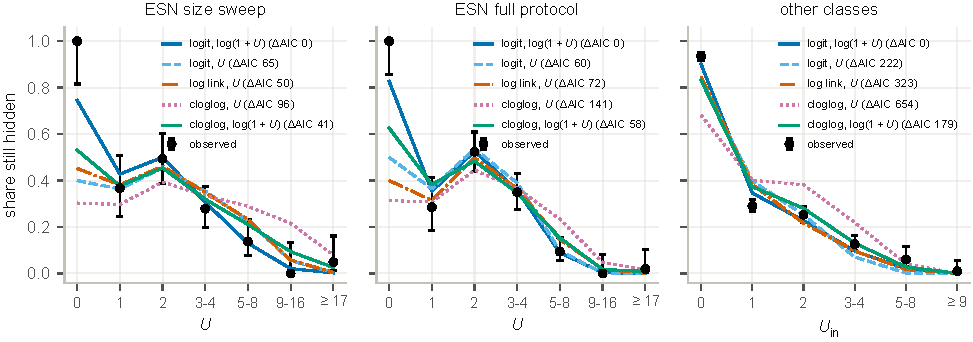
\includegraphics[width=\textwidth]{figures/sm_links.pdf}
\caption{Observed survival (dots, Wilson intervals) and the binned predictions of five fitted models.}
\label{fig:sm_links}
\end{figure*}

\section{Single equilibria and correlation within a model}

The survival of an attractor is the probability that none of the unstable equilibria of its model excites it. A logistic
model of the $9106$ pairs (unstable equilibrium, reproduced attractor) of $2431$ perceptrons and residual networks, with
covariates for the position inside $Q$, copies of true equilibria, the dimension of the unstable manifold, class, training
set, width and regime, and a random intercept per model, gives a standard deviation of the random intercept of $1.73$
$[1.58,1.90]$, a latent intra-model correlation of $0.48$ and a median odds ratio of $5.2$ (likelihood ratio against no
random intercept $1095$). The population-averaged probability that an equilibrium excites the attractor is $0.64$ ($0.68$
inside $Q$, $0.39$ outside); being inside $Q$ raises the log-odds by $1.69\pm0.13$, a copy of a true equilibrium lowers them by
$1.52\pm0.15$, and HE1 lowers them by $1.50$. The implied probability that no equilibrium of a model excites the attractor
reproduces the observed survival curve (Fig.~\ref{fig:sm_eq}; sum of squared standardized residuals over six bins $16.4$),
which independent equilibria ($106.5$) and a constant probability per equilibrium ($349$) do not. Per regime the fit is
poorer in Chua~I, Chua~II and SE11, where it predicts too few survivors at $\Uin=1$.

\begin{figure}
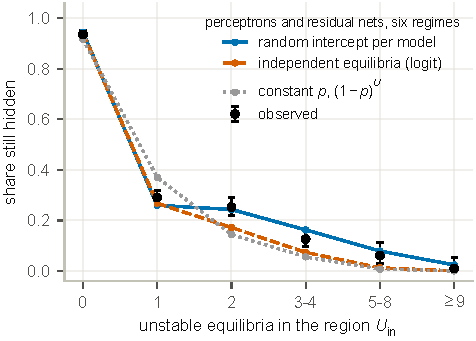
\includegraphics[width=0.6\columnwidth]{figures/sm_eq_model.pdf}
\caption{Survival of perceptrons and residual networks against $\Uin$ and the predictions of the equilibrium-level model
with a random intercept per model, with independent equilibria, and with a constant probability per equilibrium.}
\label{fig:sm_eq}
\end{figure}

\section{Sensitivity of the main fits}

\emph{Size of $Q$.} Recomputing $\Uin$ with the region scaled about its center by $s$ gives slopes of $-2.74$, $-3.62$,
$-3.94$, $-3.99$ and $-4.06$ for $s=0.5$, $0.75$, $1$, $1.5$ and $2$ in the classes, and $-2.97$, $-3.18$, $-3.54$, $-3.65$ and
$-4.27$ in the full-protocol ensemble (Fig.~\ref{fig:sm_q}). Halving $Q$ drops equilibria of its outer part, and survival at
$\Uin=0$ falls to $0.74$; for $s\ge0.75$ the slope is stable.

\emph{Reproduction thresholds.} With both thresholds on $\Delta_{\mathrm{att}}$ and $d_H$ set to $0.1$, $0.2$ and $0.3$ the
classes give $2655$, $3329$ and $3771$ reproduced pairs and slopes of $-3.69\pm0.16$, $-3.94\pm0.15$ and $-4.06\pm0.14$; the
size sweep gives $364$, $381$ and $382$ pairs and $-3.25$, $-3.08$ and $-3.08$.

\emph{Excitation at a finite radius.} Attractors excited from a ball of radius $10^{-4}$ or $10^{-3}$ but not $10^{-6}$ are
rare: $5$ of $381$ pairs in the size sweep, $10$ of $581$ networks of the full-protocol ensemble and $14$ of $3329$ pairs in
the classes. Counting them as hidden changes the slopes to $-3.04$, $-3.34$ (by $U$; $-2.97$ by $\Uin$) and $-3.88$, and no
binned share by more than $0.04$. Table~\ref{tab:sm_labels} gives the labels of the full protocol by $U$.

\emph{Reservoir spectral radius.} In the full-protocol ensemble the mean $U$ is $6.3$, $5.5$ and $8.6$ for $\rho=0.6$, $0.9$
and $1.2$; paired by seed, $\rho=1.2$ adds $3.9$ unstable equilibria on average ($82$ networks up, $16$ down). Networks with
$\rho=1.2$ reproduce the attractor less often ($41$ of $108$, against $266$ of $308$ and $274$ of $331$), and at fixed $U$ the
spectral radius has no detectable effect on survival.

\begin{figure}
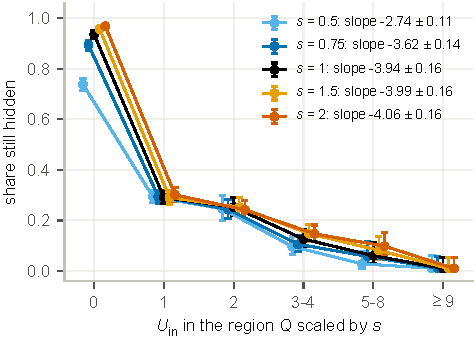
\includegraphics[width=0.6\columnwidth]{figures/sm_q_scale.pdf}
\caption{Survival of perceptrons and residual networks against $\Uin$ counted in the region $Q$ scaled about its center by
$s$, with the fitted slopes.}
\label{fig:sm_q}
\end{figure}

\begin{table}
\caption{Labels of the full protocol by the number $U$ of unstable equilibria, echo state networks of the full-protocol
ensemble, six regimes (one row per network).}
\label{tab:sm_labels}
\begin{ruledtabular}
\begin{tabular}{lrrrrr}
$U$ & $n$ & stat.\ hidden & self-excited & excited at $r>10^{-6}$ & undetermined \\
\hline
0 & 23 & 23 & 0 & 0 & 0 \\
1 & 56 & 16 & 39 & 1 & 0 \\
2 & 126 & 66 & 60 & 0 & 0 \\
3-4 & 143 & 50 & 88 & 5 & 0 \\
5-8 & 139 & 13 & 124 & 2 & 0 \\
9-16 & 43 & 0 & 42 & 1 & 0 \\
$\ge$17 & 51 & 1 & 49 & 1 & 0 \\
\end{tabular}
\end{ruledtabular}
\end{table}


\section{Fidelity of the models}

The comparison with the true system uses the uniform census points of $Q$ stored with every model. A census point is counted
as correct if its outcome in the model corresponds to its true outcome: the true hidden attractor to the model attractor that
reproduces it, a true stable equilibrium to a stable copy of it, escape to escape, and, in Chua~II, the visible cycle to an
oscillation other than the reproduced attractors (an approximation, since cycles are not matched). Agreement is counted over
the points that stay bounded in the true system. Recall is the share of the true hidden basin that reaches the reproduced
attractor. A reproduction is faithful if the model has a stable copy of the visible equilibrium, the recall is at least
$0.5$ and the model basin restricted to bounded points is within a factor of two of the true one.

Table~\ref{tab:sm_pB} and Fig.~\ref{fig:sm_fid}(a) compare the basins. In Chua~I the model basins are about ten times the
true ones, but on the points that stay bounded in the true system the ratio is close to one: the models attach to the hidden
attractor the region from which the true system escapes ($92\%$ of their basin). In Chua~II, where nothing escapes,
perceptrons trained on H1 have basins $130$ to $160$ times too large, and HE1 brings them down to a few times the true size.

Figure~\ref{fig:sm_fid}(b) splits survival by the presence of a stable copy of the visible equilibrium. Pooled over the
perceptrons and residual networks, a reproduction keeps the attractor hidden in $0.54$ of the cases with the copy and $0.29$
without, but stratified by regime, class, training set and $\Uin$ the association reverses (Mantel--Haenszel odds ratio
$0.34$ $[0.20,0.57]$); for echo state networks it is positive (odds ratio $4.7$ $[1.3,17.6]$ in the full-protocol ensemble).
Hidden and faithful are $16.5\%$ of the reproductions by perceptrons and residual networks ($27$--$45\%$ on HE1, under $1\%$ on
H1) and $4.6\%$ of those by echo state networks.

For the penalty experiment, of the $292$ unstable equilibria of index $-1$ inside $Q$ without the penalty, $285$ and $272$
disappear at $\lambda_{\mathrm{P}}=0.1$ and $1$, at most $0$ and $4$ of them could have moved out of $Q$, and the number of
equilibria falls by $283$ and $266$ pairs: the saddles are annihilated with partners. The unstable equilibria of the
penalized models are $15$ and $32$, against $650$ without the penalty.

In the intervention ensemble with imposed equilibria, all $66$ networks have index sum $1$ and all imposed copies; the copies
carry the true indices in $5$ of $16$ networks in Chua~I, $3$ of $6$ in Chua~II, $7$ of $16$ in SE3, $9$ of $16$ in SE11 and
$4$ of $6$ in each Wang--Chen regime. Where they do, the remaining equilibria have total index $1-s$: $+2$ in Chua~I (on
average $3.2$ equilibria, $1.6$ of them stable; four of the five networks have a stable one) and $0$ in Chua~II ($2.7$, none
stable). Imposed copies of stable equilibria are almost never stable (the origin of Chua~I in $0$ of $16$ networks).

\begin{table*}
\caption{Basin fraction of the reproduced hidden attractor in $Q$: true value (per attractor) and median over reproductions
for each class; in parentheses the median ratio of model to true basin restricted to points that stay bounded in the true
system. Large ratios on all of $Q$ with ratios near one on bounded points (Chua~I) mean that the model basin absorbs the
region from which the true system escapes.}
\label{tab:sm_pB}
\begin{ruledtabular}
\begin{tabular}{llllll}
Regime & true & mlp & mlp2 & res & ESN (full protocol) \\
\hline
SE3 & $0.149$ & $0.467$ ($1.00$) & $0.48$ ($1.12$) & $0.169$ ($0.89$) & $0.102$ ($0.42$) \\
SE11 & $0.007$ & $0.0683$ ($0.17$) & $0.476$ ($1.68$) & $0.0111$ ($0.55$) & $0.0175$ ($0.14$) \\
WC & $0.675$ & $0.901$ ($0.94$) & $0.876$ ($0.92$) & $0.803$ ($0.83$) & $0.562$ ($0.66$) \\
WC$'$ & $0.665$ & $0.969$ ($0.98$) & $0.969$ ($0.98$) & $0.493$ ($0.57$) & $0.53$ ($0.63$) \\
Chua~I & $0.0189$ & $0.205$ ($0.95$) & $0.238$ ($0.95$) & $0.0299$ ($1.05$) & $0.18$ ($1.01$) \\
Chua~II & $0.0012$ & $0.173$ ($157.59$) & $0.145$ ($132.18$) & $0.0039$ ($3.55$) & $0.0174$ ($15.82$) \\
LE1 & $0.0013$ & $0.0763$ ($1.42$) & $0.273$ ($1.31$) & $0.00555$ ($0.23$) & $0.0283$ ($0.46$) \\
\end{tabular}
\end{ruledtabular}
\end{table*}


\begin{figure*}
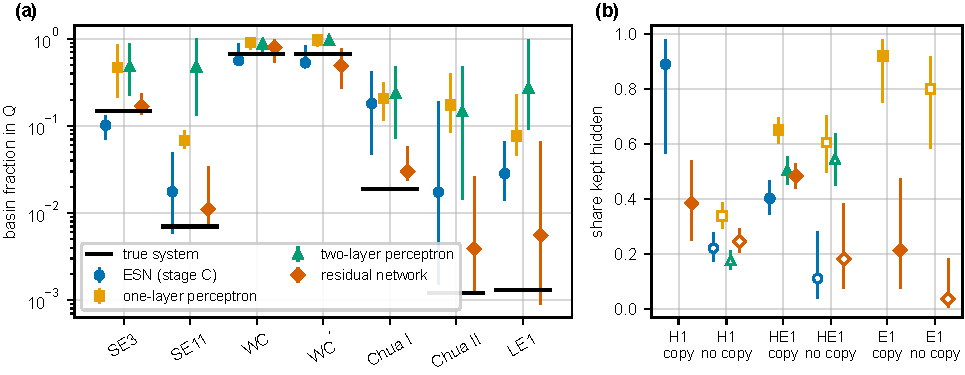
\includegraphics[width=\textwidth]{figures/sm_fid_basins.pdf}
\caption{(a) Basin fraction of the reproduced hidden attractor in $Q$ by regime and class (median and interquartile range)
against the true value (black bars). (b) Share of reproductions kept hidden with (filled) and without (open) a stable copy
of the visible equilibrium, by training set; colors as in (a).}
\label{fig:sm_fid}
\end{figure*}

\section{Which equilibria excite the attractor}

\emph{Matched null.} An unstable equilibrium inside $Q$ excites the reproduced attractor in $0.62$ of the cases for
perceptrons and residual networks and in $0.62$ for echo state networks, against $0.48$ and $0.35$ for census points of $Q$
at the same distance from the attractor that lie in its basin. The excess is large in Chua~I ($0.56$ against $0.20$), Chua~II
($0.61$ against $0.17$) and SE11, and absent for perceptrons in the Wang--Chen regimes and SE3 ($0.71$ against $0.73$, $0.61$
against $0.63$, $0.78$ against $0.70$).

\emph{Distance.} Excitation falls with the distance to the attractor in units of its diameter $D$: $1.0$ below $0.01D$
($24$ equilibria), $0.88$ between $0.01D$ and $0.03D$, about $0.6$ between $0.03D$ and $D$, and $0.28$ beyond $D$
(Fig.~\ref{fig:sm_mech}(a)).

\emph{Rotation.} The hidden attractors of SE3, SE11 and the Wang--Chen regimes rotate around the true stable equilibrium,
which lies on the rotation axis ($0.05D$ to $0.13D$ from the rotation center); there is no equilibrium-free rotation center.
Exciting equilibria are not closer to the center than the others ($0.23D$ against $0.19D$), and being encircled by the
attractor does not raise excitation (Fig.~\ref{fig:sm_mech}(b); at fixed distance it lowers the log-odds by $1.11\pm0.07$).

\emph{Spectrum.} Unstable foci (a complex pair outside the unit circle, two-dimensional unstable manifold, index $+1$) excite
more often than saddles with one real eigenvalue above one ($0.67$ against $0.55$; $0.68$ against $0.58$ for echo state
networks), and equilibria whose only unstable eigenvalue is below $-1$ excite in $0.27$.

\emph{Basin boundary.} $77\%$ of the exciting equilibria of perceptrons and residual networks, and $82\%$ of those of echo
state networks, send part of a small ball to an outcome other than the attractor, as equilibria on a basin boundary do; the
others send at least $99\%$ of the ball to the attractor ($38\%$ of exciting unstable foci, $12\%$ of exciting saddles).

\begin{figure*}
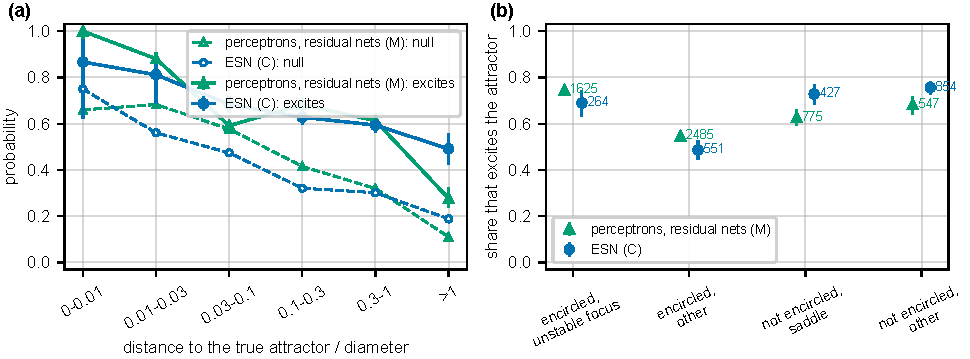
\includegraphics[width=\textwidth]{figures/sm_fid_mechanism.pdf}
\caption{(a) Share of unstable equilibria that excite the reproduced attractor (solid) and share of census points in its
basin (dashed, matched null) against the distance to the true attractor in units of its diameter. (b) Share of exciting
equilibria by type and by whether the attractor encircles the equilibrium, in the regimes with rotating attractors; numbers:
equilibria.}
\label{fig:sm_mech}
\end{figure*}

\section{Completeness of the equilibrium sets}
\label{sec:sm_complete}

Newton's method does not guarantee that all equilibria are found, and the number of equilibria of an echo state network can
grow quickly with $N$. A missed unstable equilibrium lowers $U$ and can make an attractor look hidden. The index-sum check
of the main text detects an incomplete set unless a pair of equilibria of opposite index is missed. We report three further
checks; the numbers come from \texttt{paper\_completeness.py}.

\emph{Search phases of the full protocol.} In the $868$ echo state networks of the six regimes in the full-protocol ensemble
($N=300$--$1000$, $\rho=0.6$, $0.9$, $1.2$), the search starts from uniform points of the reservoir cube, training states
and the images of the true equilibria, and continues with Newton runs on segments between attractors and stable
equilibria and with $1000$ deflated starts. All $6851$ equilibria except three were found from the initial starting
points; two were found only by deflation and one only on a segment, all three in networks with $\rho=1.2$. The
$6.8\times10^6$ Newton runs started near the basin boundaries of $341$ candidate hidden attractors (Appendix of the main
text) found no new equilibrium.

\emph{More starting points.} We rebuilt $184$ echo state networks: a stratified subsample of the size sweep ($\rho=0.9$;
$48$ networks for each of $N=100$ and $300$, $24$ for $N=700$ and $8$ for each of $N=1400$ and $2000$) and $48$ networks
with $\rho=1.2$ and $N=300$ of the full-protocol ensemble, from the six regimes, preferring networks that reproduce the
hidden attractor. Each network was rebuilt by the same training call (largest relative difference of the training error
$5\times10^{-7}$). The search of the size sweep was repeated with the same random numbers, and then with independent
blocks of starting points of the same composition, deflated against all equilibria found before, up to four ($N\ge700$) or
eight ($N\le300$) times the original number of starts. The repeated original search reproduces the stored numbers of
equilibria and unstable equilibria and the index sum in $135$ of the $136$ networks of the size sweep, and whether each
attractor is excited in all of them; in one network (SE11, $N=700$) the stored set contains a pair of equilibria of
opposite index that the rebuilt network does not show even with four times the starts.

Table~\ref{tab:sm_sat} gives the results. With $\rho=0.9$ no network gains an equilibrium, up to $N=2000$, where the
networks have $33$ unstable equilibria on average and the four searches take about four hours per network on an A100 GPU.
With $\rho=1.2$, eight times the starts find one further unstable equilibrium in two of the $48$ networks. Compared with the
stored full-protocol sets of these $48$ networks, two networks gain one unstable equilibrium each: in one the stored set
had index sum $0$, was flagged as incomplete and is therefore excluded from the survival analyses; in the other the stored
set passed the index-sum check, and the new equilibrium shows that it is incomplete. Neither network reproduces the hidden
attractor. Of the $120$ reproduced attractors, the $23$ that no equilibrium found by the original search excites stay
not excited with all starts; the one newly found unstable equilibrium that excites a reproduced attractor does so in a
network where the attractor was already self-excited.

\begin{table*}
\caption{Saturation of the equilibrium search of echo state networks. Networks rebuilt from the size sweep ($\rho=0.9$) and
from the full-protocol ensemble ($\rho=1.2$), six regimes. $\bar U$: mean number of unstable equilibria found by the original
search; $\times2$, $\times4$, $\times8$: networks in which two, four or eight times as many Newton starts find equilibria
that the original search does not; $\Delta\bar U$: mean increase of $U$ with the largest number of starts; reproduced: reproduced
hidden attractors; not excited: of these, attractors that no unstable equilibrium found by the original search excites
(light protocol); changed: of these, attractors excited by an equilibrium found with more starts.}
\label{tab:sm_sat}
\begin{ruledtabular}
\begin{tabular}{rrrrrrrrrrr}
$N$ & $\rho$ & networks & $\bar U$ & $\times2$ & $\times4$ & $\times8$ & $\Delta\bar U$ & reproduced & not excited & changed \\
\hline
100 & 0.9 & 48 & $5.5$ & 0 & 0 & 0 & $0.00$ & 15 & 3 & 0 \\
300 & 0.9 & 48 & $3.5$ & 0 & 0 & 0 & $0.00$ & 43 & 11 & 0 \\
300 & 1.2 & 48 & $8.4$ & 1 & 1 & 2 & $0.04$ & 23 & 0 & 0 \\
700 & 0.9 & 24 & $6.0$ & 0 & 0 & -- & $0.00$ & 23 & 7 & 0 \\
1400 & 0.9 & 8 & $18.1$ & 0 & 0 & -- & $0.00$ & 8 & 2 & 0 \\
2000 & 0.9 & 8 & $32.9$ & 0 & 0 & -- & $0.00$ & 8 & 0 & 0 \\
\end{tabular}
\end{ruledtabular}
\end{table*}


\emph{Certified enumeration for the three-dimensional models.} The weights of the perceptrons and residual networks of the
main text were not stored. We retrained $960$ of them with the training code, seeds and settings of the main text and saved
the weights: one- and two-layer perceptrons with $H=64$ and $256$ and residual networks with $H=64$, trained on H1 and HE1,
in the six regimes. Of these, $720$ were trained on the A100 GPU in groups of $20$ seeds as in the main text (all classes of
SE3 and SE11, and the perceptrons with $H=256$ of the other four regimes). They coincide with the models of the main text:
the training errors are identical, and the Newton search gives the same numbers of equilibria and of unstable equilibria in
all $720$. The other $240$ models ($H=64$, four regimes) were trained on a CPU with $10$ seeds per group; their random numbers
differ, so they are new realizations of the same protocol.

For each model all fixed points were enumerated by the interval Krawczyk method with
bisection\cite{Krawczyk1969Newton,Moore2009Interval} in a box that contains all of them. For bounded models this is the
image box of the map, $b\pm\sum_k|W_{\cdot k}|$ for the last layer with weights $W$ and bias $b$, since $|\tanh|<1$.
Residual networks are unbounded; for them the box is the region $Q$ enlarged by $1\%$ of its width on each side, and in
addition the box of the Newton starts, twice as wide as $Q$. A box $X$ is discarded if it does not meet its image (bounded
models) or if the interval extension of $g(u)=u-F(u)$ excludes zero. Otherwise the Krawczyk operator
$K(X)=m-Yg(m)+\bigl(I-Yg'(X)\bigr)(X-m)$, with $m$ the midpoint of $X$ and $Y$ the inverse of the midpoint of the interval
Jacobian $g'(X)$, either excludes a zero ($K(X)\cap X=\emptyset$), proves that $X$ contains exactly one zero ($K(X)$ in the
interior of $X$), or replaces $X$ by $X\cap K(X)$, which is bisected if it shrinks by less than $30\%$. The interval
arithmetic is carried out in double precision, with every computed bound widened by an a priori bound of its rounding error.
When no box remains undecided, the certified set is complete in the box.

Table~\ref{tab:sm_cert} gives the results. The enumeration decided every box in all $960$ models, and in every model the
certified set equals the set found by Newton's method from the starting points of the main text, in $Q$ and outside it:
Newton's method missed no equilibrium. The certified sets of all $800$ bounded models have index sum $1$; those of the
residual networks in $Q$ have index sum $1$ in $93$ of $160$, since $Q$ need not contain all their equilibria. In the larger
box of the Newton starts, Newton's method missed one unstable equilibrium, outside $Q$, in one residual network, which
leaves $\Uin$ unchanged.

\begin{table*}
\caption{Certified enumeration of the fixed points of perceptrons and residual networks by the interval Krawczyk method,
compared with Newton's method from the starting points of the main text. $\bar K$, $\bar U$, $\bar U_{\mathrm{in}}$: mean
numbers of certified equilibria, unstable equilibria and unstable equilibria in $Q$; differs: models whose certified set
differs from the Newton set; missed: equilibria missed by Newton's method; undecided: models with boxes that the method
could not decide; time: wall-clock time per model in one worker process.}
\label{tab:sm_cert}
\begin{ruledtabular}
\begin{tabular}{lrrrrrrrrrr}
Class & $H$ & models & $\bar K$ & $\bar U$ & $\bar U_{\mathrm{in}}$ & differs & missed & undecided & median (s) & max (s) \\
\hline
mlp & 64 & 160 & $2.08$ & $1.04$ & $0.96$ & 0 & 0 & 0 & $0.41$ & $4.26$ \\
mlp & 256 & 240 & $1.88$ & $0.99$ & $0.97$ & 0 & 0 & 0 & $5.28$ & $30.6$ \\
mlp2 & 64 & 160 & $2.09$ & $1.14$ & $1.12$ & 0 & 0 & 0 & $36.8$ & $245$ \\
mlp2 & 256 & 240 & $3.44$ & $2.71$ & $2.70$ & 0 & 0 & 0 & $215$ & $2772$ \\
res\footnotemark[1] & 64 & 160 & $2.12$ & $1.34$ & $1.34$ & 0 & 0 & 0 & $0.17$ & $1.66$ \\
\end{tabular}
\end{ruledtabular}
\footnotetext[1]{Residual networks are unbounded; their fixed points are enumerated in $Q$ only.}
\end{table*}


\bibliography{refs}

\end{document}
